\documentclass[fleqn,11pt]{article}

\usepackage[letterpaper,margin=0.75in]{geometry}

\usepackage{amsmath}
\usepackage{booktabs}
\usepackage{graphicx}
\usepackage{listings}
\usepackage{tikz}

\setlength{\parindent}{1.4em}

\begin{document}

\lstset{
  language=Python,
  basicstyle=\small,          % print whole listing small
  keywordstyle=\bfseries,
  identifierstyle=,           % nothing happens
  commentstyle=,              % white comments
  stringstyle=\ttfamily,      % typewriter type for strings
  showstringspaces=false,     % no special string spaces
  numbers=left,
  numberstyle=\tiny,
  numbersep=5pt,
  frame=tb,
}

\title{Lab 1 Report}

\author{Martin Sanchez and Ben Jacobson}

\date{2/1/17}

\maketitle

\section{Two Nodes}

In this first section we explored a simple network consisting of two nodes and one bidirectional link. We simulated the following scenarios:
\begin{enumerate}

\item Set the bandwidth of the links to 1 Mbps, with a propagation delay of 1 second. Send one packet with 1000 bytes from n1 to n2 at time 0.

\item Set the bandwidth of the links to 100 bps, with a propagation delay of 10 ms. Send one packet witih 1000 bytes from n1 to n2 at time 0.

\item Set the bandwidth of the links to 1 Mbps, with a propagation delay of 10 ms. Send three packets from n1 to n2 at time 0 seconds, then one packet at time 2 seconds. All packets should have 1000 bytes.

\end{enumerate}
After running the simulations we will show our network configuration, the output of the simulation and the calculations we used to verify that the output was correct. 

The results of running the simulator for each of the scenarios are below:

\begin{enumerate}
  \item 
    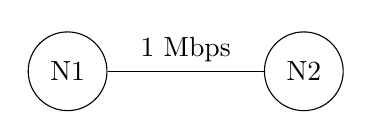
\begin{tikzpicture}
    \node[circle,draw, minimum size=1cm] (A) at (0,0) {N1};
    \node[circle,draw, minimum size=1cm] (B) at (3,0) {N2};
    \draw (A) -- (B) node[pos=0.5, sloped, above] {1 Mbps};
    \end{tikzpicture}

    The output of the simulation was:
    \begin{lstlisting} 
    Created:0  ID:1 Received: 0.009000000000000001
    \end{lstlisting}

  \item 
    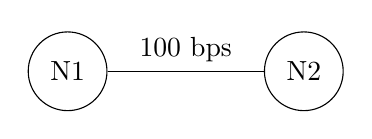
\begin{tikzpicture}
    \node[circle,draw, minimum size=1cm] (A) at (0,0) {N1};
    \node[circle,draw, minimum size=1cm] (B) at (3,0) {N2};
    \draw (A) -- (B) node[pos=0.5, sloped, above] {100 bps};
    \end{tikzpicture}

    The output of the simulation was: 
    \begin{lstlisting}
      Created:0  ID:1 Received: 80.01
    \end{lstlisting}

  \item 
    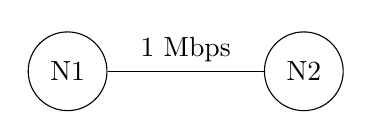
\begin{tikzpicture}
    \node[circle,draw, minimum size=1cm] (A) at (0,0) {N1};
    \node[circle,draw, minimum size=1cm] (B) at (3,0) {N2};
    \draw (A) -- (B) node[pos=0.5, sloped, above] {1 Mbps};
    \end{tikzpicture}

  The output of the simulation was:
  \begin{lstlisting}
    Created:0  ID:1  Received:0.018000000000000002
    Created:0  ID:2  Received:0.026000000000000002
    Created:0  ID:3  Received:0.034
    Created:2.0  ID:4  Received:0.017999999999999794
  \end{lstlisting}
\end{enumerate}

% \begin{lstlisting}
% class Node:
%     def __init__(self,scheduler):
%         self.scheduler = scheduler

%     def handle_message(self,t,message):
%         print "Received at",t,':',message.body
%         if message.times < 3:
%             self.scheduler.add(t+1.5, message, self.handle_message)
%         message.times += 1
% \end{lstlisting}

\section{Three Nodes}

In this section we will use the simulator to setup a network consisting of three nodes and two links. We will test two fast links and one fast link with a slow link. For each scenario we will show our network configuration, the last 5 lines of the simulation ouput and the calculations we used to verify the output.
The results are as follows.  

\begin{enumerate}
  \item 
  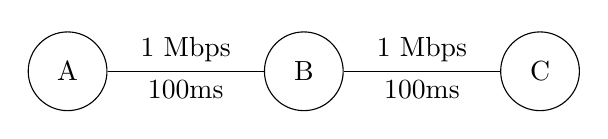
\begin{tikzpicture}
    \node[circle,draw, minimum size=1cm] (A) at (0,0) {A};
    \node[circle,draw, minimum size=1cm] (B) at (3,0) {B};
    \node[circle,draw, minimum size=1cm] (C) at (6,0) {C};
    \draw (A) -- node[pos=0.5,above] {1 Mbps} node[midway,below]{100ms}(B) -- (C) node[pos=0.5,above] {1 Mbps} node[midway,below]{100ms};
  \end{tikzpicture}

  \item 
  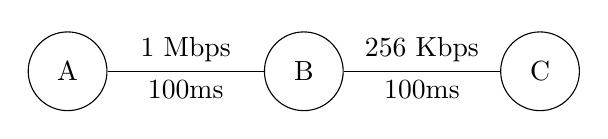
\begin{tikzpicture}
    \node[circle,draw, minimum size=1cm] (A) at (0,0) {A};
    \node[circle,draw, minimum size=1cm] (B) at (3,0) {B};
    \node[circle,draw, minimum size=1cm] (C) at (6,0) {C};
    \draw (A) -- node[pos=0.5,above] {1 Mbps}  node[midway,below]{100ms}(B) -- (C) node[pos=0.5, above] {256 Kbps}  node[midway,below]{100ms};
  \end{tikzpicture}
\end{enumerate}

% \vspace{0.5cm}
% \begin{tabular}{lc}
%   \toprule
%   Setting & Result\\
%   \midrule
%   1 & 1.0\\
%   2 & 3.45\\
%   3 & 7.85\\
%   4 & 15.89\\
%   \bottomrule
% \end{tabular}
% \vspace{0.5cm}


\section{Queueing Theory}



% \includegraphics[width=11cm]{graphs/queueing_theory}
This is the graph of our queue theory output. 
\section{Summary}

% $d_{trans}$ is the transmission delay. $d_{prop}$ is the propagation delay.

% \begin{align*}
% d &= d_{trans} + d_{prop}\\
%   &= (1000*8)/1000000 + 0.05\\
%   &= 0.058
% \end{align*}

\end{document}